\usepackage{minted}

\date{Nordic Perl Workshop 2018, Oslo, 6th September}

\begin{document}
\maketitle

\begin{frame}
  \titlepage
\end{frame}

\cleardoublepage

\tableofcontents

\cleardoublepage

\section{Introduction}

Text versus:

\begin{itemize}
\item HTML
\item Attachments
\item Embedded Images
\end{itemize}

Challenges:

Secluded island.


\begin{itemize}
  \item Security
  \item Encryption
  \item SPAM
  \item Virus
  \item Counter Measures
\end{itemize}

So it is a jungle and we literally need to hack our way through it.

\begin{frame}{Email with Perl}
  % https://pixabay.com/en/swamp-marsh-green-nature-landscape-1706114/
  \begin{figure}[!ht]
    \centering
    
\includegraphics[width=0.9\linewidth]{img/swamp-1706114_1920.jpg}
  \end{figure}
\end{frame}

\section{Overview}

\begin{frame}{Overview}
  \begin{itemize}
  \item Email structure
  \item Sending emails
  \item IMAP
  \item Parsing emails
  \item Use Cases  
  \end{itemize}
\end{frame}

\section{Email structure}

Gone are the days of plain text emails, the majority is written in HTML with
a plain text equivalent if you are lucky.

\begin{frame}{Email structure}
  \begin{itemize}
  \item Header
  \item Body
  \end{itemize}
\end{frame}

\begin{frame}{Email structure}
  \begin{itemize}
  \item Attachments
  \item HTML / Plaintext
  \end{itemize}
\end{frame}

A very nice feature of the Email::MIME module (more about that later)
is the \verb|debug_structure| method which gives you an overview about the
different parts forming the email body.

\begin{frame}[fragile]{Email structure}
\begin{minted}{perl}
Email::MIME->new( $message )->debug_structure;
\end{minted}
\end{frame}

\begin{frame}[fragile]{Email structure}
\begin{lstlisting}
+ multipart/mixed;
    + application/octet-stream; name=83AKE9.pdf
    + multipart/alternative;
        + text/plain; charset=UTF-8
        + text/html; charset=UTF-8
\end{lstlisting}
\end{frame}

\section{Sending emails}

\begin{frame}{Sending emails}
  % https://pixabay.com/en/wealth-currency-paper-abundance-3262562/
  Too many ways to do it ...
  \begin{figure}[!ht]
    \centering
    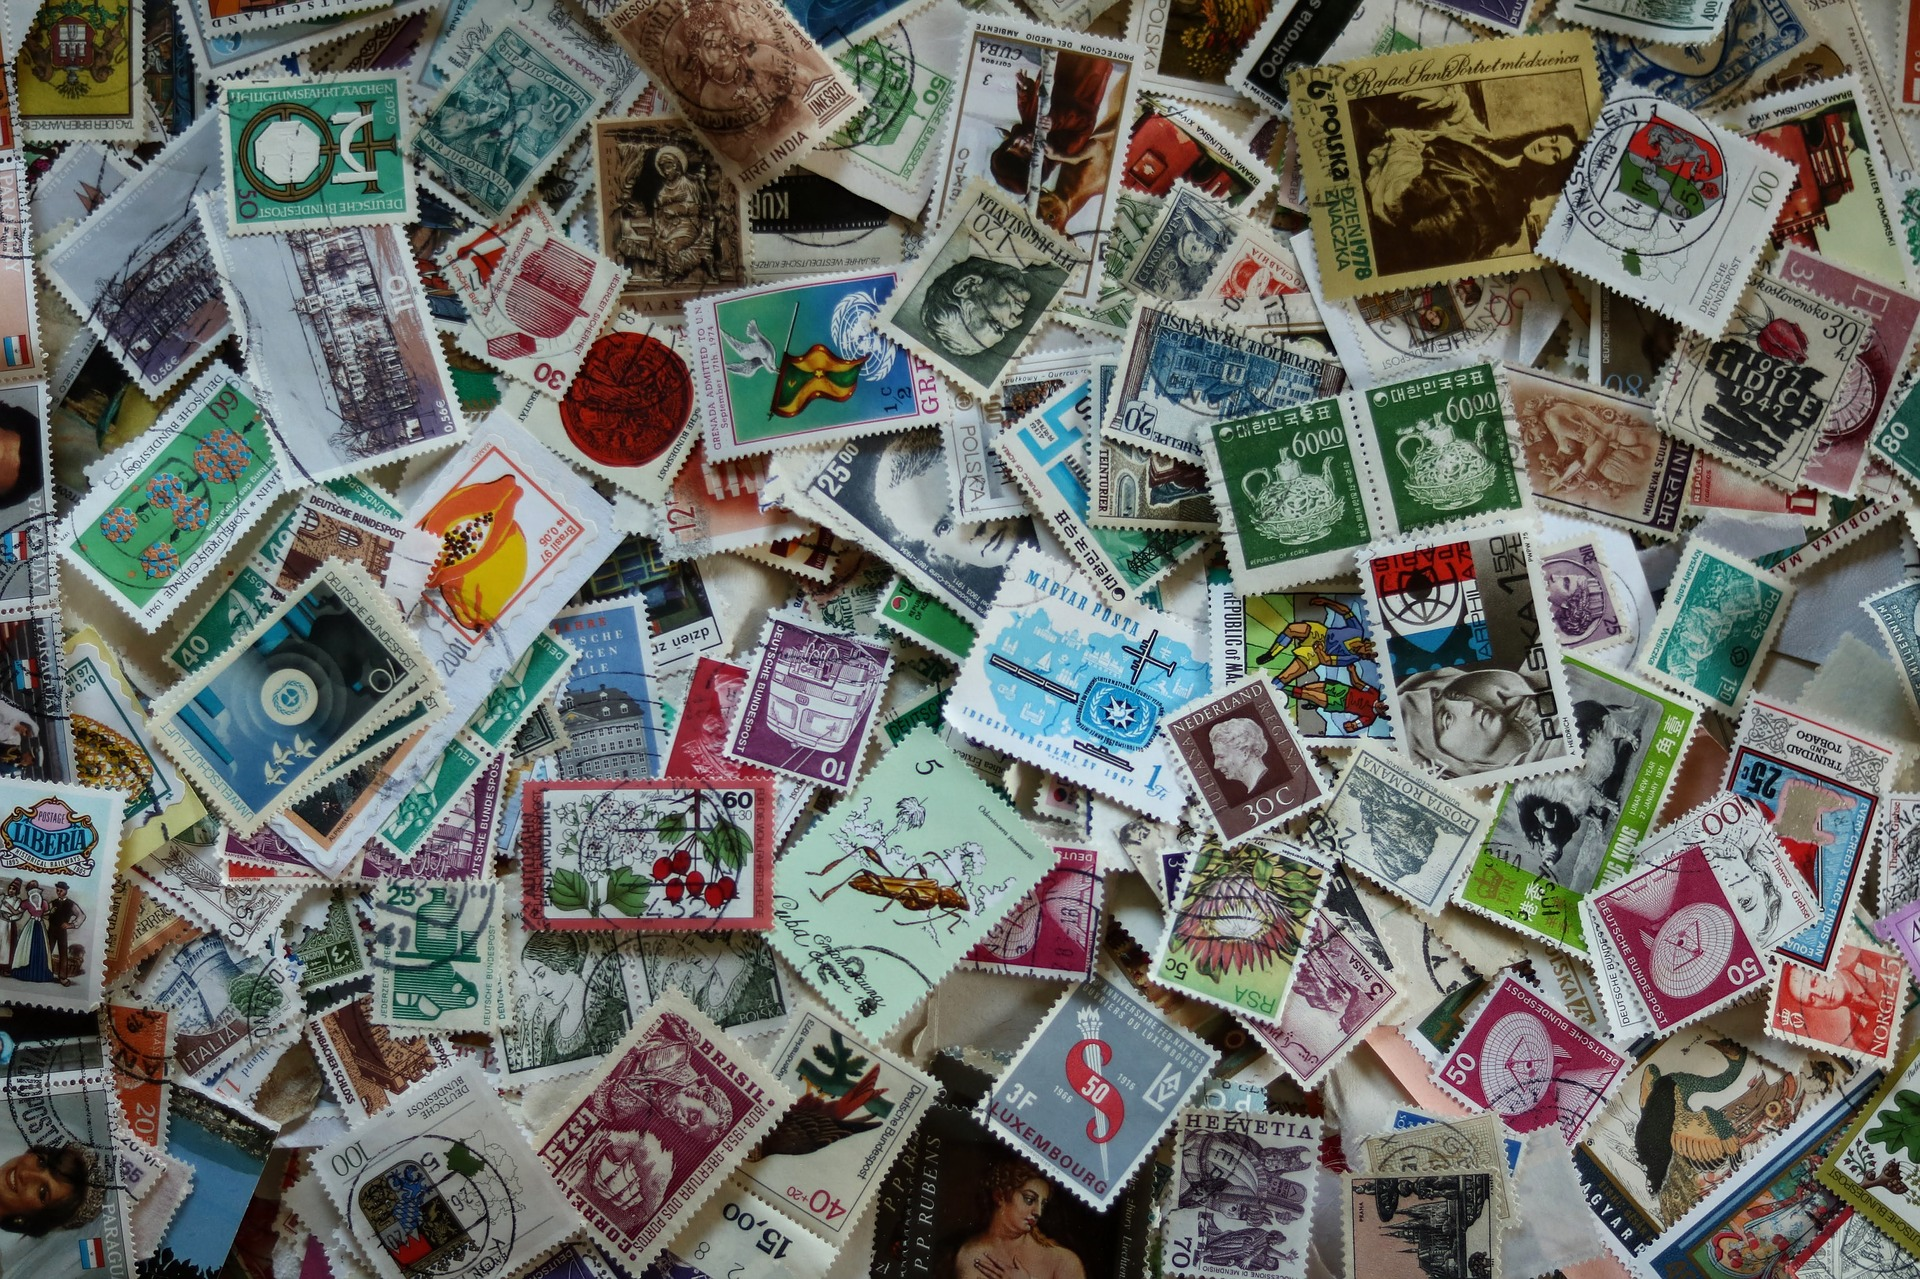
\includegraphics[width=0.9\linewidth]{img/wealth-3262562_1920.jpg}
  \end{figure}
\end{frame}

\begin{frame}{Module (Legacy)}
  \begin{itemize}
    \item Net::SMTP
    \item MIME::Lite
  \end{itemize}
\end{frame}

\begin{frame}{Module}
  Send:

  \begin{itemize}
  \item Email::Send (deprecated)
  \item Email::Sender
  \item Email::Sender::Simple
  \end{itemize}

  Misc:

  \begin{itemize}
  \item Email::MIME
  \item MIME::Entity
  \item Mail::Box
  \end{itemize}

\end{frame}

\begin{lstlisting}
use Email::Sender::Simple qw(sendmail);
use Email::Simple;
use Email::Simple::Creator;
\end{lstlisting}

\begin{frame}[fragile]{Example}
  \begin{minted}{perl}
my $email = Email::Simple->create(
    header => [
        From    => '"Module Updates" <info@cpan.pm>',
        To      => '"Racke" <racke@racke.pm>',
        Subject => 'Changes in Module Foo::Bar',
    ],
    body => "Baz.\n",
);

sendmail($email);
  \end{minted}
\end{frame}

Email::Simple unfortunately lacks a method for attachments. So we are simply
using MIME::Entity instead.

\begin{frame}[fragile]{Example with attachment}
\begin{minted}{perl}

my $email = MIME::Entity->build(
    From    => '"Module Updates" <info@cpan.pm>',
    To      => '"Racke" <racke@racke.pm>',
    Subject => 'Changes in Module Foo::Bar',
    Data => ["Baz.\n"],
);

$email->attach(
    Path => '../perlmail-de-handout.pdf',
    Type => 'application/pdf',
);

sendmail($email);
  \end{minted}
\end{frame}

\begin{frame}[fragile]{Example with umlaut}
  \begin{minted}{perl}
my $email = Email::Simple->create(
    header => [
        From    => '"Module Updates" <info@cpan.pm>',
        To      => '"Racke" <racke@racke.pm>',
        Subject =>  'Änderungen im Modul Foo::Bar',
    ],
    body => "Baz.\n",
);

sendmail($email);
  \end{minted}
\end{frame}

\begin{frame}[fragile]{Mail Clients}

  \begin{itemize}
  \item[\goodsmile] Thunderbird
  \item[\sadsmile] K9 (Android)
  \end{itemize}

\end{frame}

\begin{frame}[fragile]{Correction: Example with umlaut}
  \begin{minted}{perl}
my $email = Email::Simple->create(
    header => [
        From    => '"Module Updates" <info@cpan.pm>',
        To      => '"Racke" <racke@racke.pm>',
        Subject => encode('MIME-Header', 
                          'Änderungen im Modul Foo',
                         ),
    ],
    body => "Bar.\n",
);

sendmail($email);
  \end{minted}
\end{frame}

\begin{frame}[fragile]{Encoded subject}
  \begin{lstlisting}
To: "Racke" <racke@racke.pm>
From: "Module Updates" <info@cpan.pm>
Subject: =?UTF-8?B?w4RuZGVydW5nZW4gaW4gTW9kdWxlIEZvbw==?=
\end{lstlisting}
\end{frame}

\begin{frame}[fragile]{Encoding email body}
  \begin{minted}{perl}
my $email = Email::Simple->create(
    header => [
        From    => '"Module Updates" <info@cpan.pm>',
        To      => '"Racke" <racke@racke.pm>',
        Subject => encode('MIME-Header',
                          'Änderungen im Modul Foo::Bar',
                         ),
    ],
    body => encode('UTF-8', "Überflüssig"),
);

sendmail($email);
  \end{minted}
\end{frame}

\subsection{Transports}

\begin{frame}{Transports}
  % https://pixabay.com/en/sunset-plane-take-off-nature-3193002/
  \begin{figure}[!ht]
    \centering
    
\includegraphics[width=0.9\linewidth]{img/sunset-3193002_1920.jpg}
  \end{figure}
\end{frame}

\begin{frame}{Transports}
  \begin{itemize}
    \item Sendmail
    \item SMTP
    \item Maildir
%    \item Test
    \item Redirect
  \end{itemize}
\end{frame}

\subsubsection{Sendmail-Transport}

Wenn nicht anders angegeben, wird der Sendmail-Transport verwendet, d.h. der
auf dem Rechner installierte Mailserver.

Das ist nicht immer erwünscht, z.B. wegen dynamischer IP oder vorgebener
Mailserver.

\begin{frame}[fragile]{Sendmail-Transport}
\begin{minted}{perl}
sendmail( $email );
\end{minted}
\end{frame}

\subsubsection{Maildir-Transport}

Beim Maildir-Transport wird das Verzeichnis Maildir im aktuellen Verzeichnis
verwendet und angelegt soweit nicht vorhanden.

Deshalb verwenden wir hier das Verzeichnis Maildir im Homeverzeichnis.

\begin{lstlisting}
use Email::Sender::Transport::Maildir qw();
use File::HomeDir;
use Path::Tiny;
\end{lstlisting}

\begin{frame}[fragile]{Maildir-Transport}
  \begin{minted}{perl}

my $maildir = path(File::HomeDir->my_home)
    ->child('Maildir');

my $transport = Email::Sender::Transport::Maildir->new(
   dir => $maildir
);

sendmail( $email , { transport => $transport, } );

\end{minted}
\end{frame}

\subsubsection{Test-Transport}

%\begin{frame}[fragile]{Test-Transport}
\begin{minted}{perl}

\end{minted}
%\end{frame}

\subsubsection{Redirect-Transport}

\begin{frame}[fragile]{Redirect-Transport}
  \begin{minted}{perl}

$transport_orig = Email::Sender::Transport::Sendmail->new;

$transport = Email::Sender::Transport::Redirect->new({
  transport => $transport_orig,
  redirect_address => 'racke@linuxia.de',
});

sendmail( $email , { transport => $transport, } );

\end{minted}
\end{frame}

\begin{frame}[fragile]{Redirect-Transport}
\begin{lstlisting}
To: racke@linuxia.de
Cc: racke@linuxia.de
From: "Module Updates" <info@cpan.pm>
Subject: Hello world!
Date: Tue, 3 Apr 2018 08:45:59 +0200
X-Intercepted-To: "Racke" <racke@racke.pm>
X-Intercepted-Cc: "Info" <info@racke.pm>
X-Email-Sender-From: info@cpan.pm
X-Email-Sender-To: racke@linuxia.de
X-Email-Sender-To: racke@linuxia.de
Lines: 1

Here we go.
\end{lstlisting}
\end{frame}

\subsection{Embedding images}

\begin{frame}{Embedding images}
  \begin{itemize}
  \item Images as links
  \item Base64 encoded
  \item CID Inline
  \end{itemize}
\end{frame}


\subsection{Create emails from templates}

\begin{frame}[fragile]{Emails from templates}
  \begin{minted}{perl}
    my $html = template $template, $tokens,
       { layout => 'email' };

    my $f    = HTML::FormatText::WithLinks->new;
    my $text = $f->parse($html);
  \end{minted}
\end{frame}

Dancer::Plugin2::Email uses MIME::Entity and Email::Sender.

\begin{frame}[fragile]{Emails from templates}
\begin{minted}{perl}
  email {
      %args,
      body   => encode( 'UTF-8', $text ),
      type   => 'text',
      attach => {
         Charset  => 'utf-8',
         Data     => encode( 'UTF-8', $html ),
         Encoding => "quoted-printable",
         Type     => "text/html"
      },
      multipart => 'alternative',
  };
\end{minted}
\end{frame}

\section{IMAP}

\begin{frame}{IMAP}
  \begin{itemize}
  \item Modules
  \item Login
  \item Select folder
  \item Search emails
  \item Download emails
  \end{itemize}
\end{frame}

\subsection{IMAP Modules}

\begin{frame}{IMAP Modules}
  \begin{itemize}
  \item Net::IMAP::Client
  \item Net::IMAP::Simple
  \end{itemize}
\end{frame}

\begin{frame}[fragile]{Differences between IMAP modules}
  \begin{itemize}
  \item Constructor
    \begin{itemize}
      \item server
      \item ssl / use\_ssl
    \end{itemize}
  \item Supported methods
  \item Return values
    \begin{itemize}
    \item select
      \item search
    \end{itemize}
  \end{itemize}
\end{frame}

\subsection{Login}

\begin{frame}[fragile]{Login}
\begin{minted}{perl}
my $imap = Net::IMAP::Client->new(
    server => 'mail.linuxia.pm',
    ssl => 1,
    port => 993,
    user => 'racke@racke.pm',
    pass => 'nevairbe',
);

$imap->login;
\end{minted}
\end{frame}

login rejected

\subsection{Select folder}

IMAP servers use different separators for the folder hierarchy.

\begin{frame}[fragile]{Select folder}
  Select folder (Dbmail):

\begin{minted}{perl}
  $imap->select('INBOX/Consulting/Bahn');
\end{minted}

  Select folder (Courier):

\begin{minted}{perl}
  $imap->select('INBOX.Consulting.Bahn');
\end{minted}

\end{frame}

\begin{frame}[fragile]{Folder separator}

\begin{minted}{perl}
  $imap->separator;
\end{minted}

\end{frame}

\subsection{Search emails}

It is mandatory to select a folder first, otherwise the search fail with an
error message like \verb|Error in IMAP command received by server|.

\begin{frame}[fragile]{Search emails}
  Search emails in selected folder:

\begin{minted}{perl}
  $ids = $imap->search( { subject => 'Perl' }, 'DATE' );
\end{minted}
\end{frame}

\subsection{Processing emails}

\begin{frame}[fragile]{Processing emails}
  Download complete email:

\begin{minted}{perl}
$message = $imap->get_rfc822_body($id);
\end{minted}
\end{frame}

\section{Processing emails}

\begin{frame}{Modules for processing}
  \begin{itemize}
  \item Email::MIME
  \item Email::Simple
  \end{itemize}
\end{frame}

\begin{frame}[fragile]{Email::MIME}
  \begin{itemize}
    \item Read Email from IMAP:

\begin{minted}{perl}
my $message = $imap->get_rfc822_body($id);
\end{minted}

  \item Read email from file:

\begin{minted}{perl}
use IO::All;
my $message = io->file('email.eml')->all;
\end{minted}

  \item Parse email:

\begin{minted}{perl}
my $parser = Email::MIME->new($message);
\end{minted}

\end{itemize}  
\end{frame}

\begin{frame}[fragile]{Email::MIME}
  Subject header:

\begin{minted}{perl}
$parser->header_str('Subject');
\end{minted}

\end{frame}

The header will be already decoded.

\begin{frame}[fragile]{Email::MIME}
Walk MIME parts:

\begin{minted}{perl}
my @out;

$parser->walk_parts(sub {
  my ($part) = @_;
  return if $part->subparts;

  if ($part->content_type =~ m{text/html}i) {
    push @out, $part->body_str;
  }
});
\end{minted}
\end{frame}

\subsection{Extract train ticket}

\begin{frame}[fragile]{Extract train ticket}
\begin{minted}{perl}

$ids = $imap->search('FROM buchungsbestaetigung@bahn.de');

for my $imap_id (@$ids) {
    my $message = $imap->get_rfc822_body($imap_id);
    my $parser = Email::MIME->new($message);
    my @out;

    ...
}

\end{minted}
\end{frame}

\begin{frame}[fragile]{Extract train ticket}
\begin{minted}{perl}
$parser->walk_parts(
  sub {
    my ($part) = @_;
    return if $part->subparts;

    if ($part->content_type =~ m{application/octet-stream}i){
      push @out, [ $part->filename, $part->body ];
    }
  }
);

$out[0][1] > io($out[0][0]);
\end{minted}
\end{frame}

\section{Use Cases}

\begin{frame}{Use Cases}
  \begin{itemize}
  \item Dancer2::Plugin::Email (Email::Sender)
  \item Helpdesk::Integration
  \item Sympa
  \item Spamassassin
  \end{itemize}
\end{frame}

\subsection{Helpdesk::Integration}

\begin{frame}{Helpdesk::Integration}
  \begin{itemize}
  \item Request Tracker
    \begin{itemize}
    \item Web-Interface
    \item Email-Interface
    \end{itemize}
  \end{itemize}
\end{frame}

\begin{frame}{Helpdesk::Integration}
  \begin{itemize}
  \item Search IMAP folder
  \item Parse emails
  \item Create/update ticket through REST API
  \end{itemize}
\end{frame}

\section{Finish}

\subsection{Questions}

\begin{frame}{Questions}
% https://pixabay.com/de/fragezeichen-wissen-frage-anmelden-3255140/
  \begin{figure}[!ht]
     \centering
     
\includegraphics[width=0.9\linewidth]{img/question-mark-3255140_1920.jpg}
  \end{figure}
\end{frame}

\subsection{The end}

\begin{frame}{The end}
% https://pixabay.com/de/ortsschild-ortstafel-schluss-aus-1158385/
  \begin{figure}[!ht]
     \centering
     
\includegraphics[width=0.8\linewidth]{img/town-sign-1158385_1920.jpg}
  \end{figure}
\end{frame}

\end{document}

%%% Local Variables: 
%%% mode: latex
%%% TeX-master: t
%%% End: 
